%% This is file `elsarticle-template-1-num.tex',
%%
%% Copyright 2009 Elsevier Ltd
%%
%% This file is part of the 'Elsarticle Bundle'.
%% ---------------------------------------------
%%
%% It may be distributed under the conditions of the LaTeX Project Public
%% License, either version 1.2 of this license or (at your option) any
%% later version.  The latest version of this license is in
%%    http://www.latex-project.org/lppl.txt
%% and version 1.2 or later is part of all distributions of LaTeX
%% version 1999/12/01 or later.
%%
%% The list of all files belonging to the 'Elsarticle Bundle' is
%% given in the file `manifest.txt'.
%%
%% Template article for Elsevier's document class `elsarticle'
%% with numbered style bibliographic references
%%
%% $Id: elsarticle-template-1-num.tex 149 2009-10-08 05:01:15Z rishi $
%% $URL: http://lenova.river-valley.com/svn/elsbst/trunk/elsarticle-template-1-num.tex $
%%
\documentclass[preprint,12pt]{elsarticle}

%% Use the option review to obtain double line spacing
%% \documentclass[preprint,review,12pt]{elsarticle}

%% Use the options 1p,twocolumn; 3p; 3p,twocolumn; 5p; or 5p,twocolumn
%% for a journal layout:
%% \documentclass[final,1p,times]{elsarticle}
%% \documentclass[final,1p,times,twocolumn]{elsarticle}
%% \documentclass[final,3p,times]{elsarticle}
%% \documentclass[final,3p,times,twocolumn]{elsarticle}
%% \documentclass[final,5p,times]{elsarticle}
%% \documentclass[final,5p,times,twocolumn]{elsarticle}

%% if you use PostScript figures in your article
%% use the graphics package for simple commands
%% \usepackage{graphics}
%% or use the graphicx package for more complicated commands
%% \usepackage{graphicx}
%% or use the epsfig package if you prefer to use the old commands
%% \usepackage{epsfig}

%% The amssymb package provides various useful mathematical symbols
\usepackage{amssymb}
%% The amsthm package provides extended theorem environments
%% \usepackage{amsthm}

%% The lineno packages adds line numbers. Start line numbering with
%% \begin{linenumbers}, end it with \end{linenumbers}. Or switch it on
%% for the whole article with \linenumbers after \end{frontmatter}.
\usepackage{lineno}

%% natbib.sty is loaded by default. However, natbib options can be
%% provided with \biboptions{...} command. Following options are
%% valid:

%%   round  -  round parentheses are used (default)
%%   square -  square brackets are used   [option]
%%   curly  -  curly braces are used      {option}
%%   angle  -  angle brackets are used    <option>
%%   semicolon  -  multiple citations separated by semi-colon
%%   colon  - same as semicolon, an earlier confusion
%%   comma  -  separated by comma
%%   numbers-  selects numerical citations
%%   super  -  numerical citations as superscripts
%%   sort   -  sorts multiple citations according to order in ref. list
%%   sort&compress   -  like sort, but also compresses numerical citations
%%   compress - compresses without sorting
%%
%% \biboptions{comma,round}

% \biboptions{}


\usepackage{polski}
\usepackage[utf8]{inputenc}
\usepackage{enumitem}

%%\journal{Journal Name}

\begin{document}

\begin{frontmatter}

%% Title, authors and addresses

%% use the tnoteref command within \title for footnotes;
%% use the tnotetext command for the associated footnote;
%% use the fnref command within \author or \address for footnotes;
%% use the fntext command for the associated footnote;
%% use the corref command within \author for corresponding author footnotes;
%% use the cortext command for the associated footnote;
%% use the ead command for the email address,
%% and the form \ead[url] for the home page:
%%
%% \title{Title\tnoteref{label1}}
%% \tnotetext[label1]{}
%% \author{Name\corref{cor1}\fnref{label2}}
%% \ead{email address}
%% \ead[url]{home page}
%% \fntext[label2]{}
%% \cortext[cor1]{}
%% \address{Address\fnref{label3}}
%% \fntext[label3]{}

\title{Wykorzystanie głębokich sieci neuronowych do uczenia ze wzmocnieniem w grach komputerowych - raport}

%% use optional labels to link authors explicitly to addresses:
%% \author[label1,label2]{<author name>}
%% \address[label1]{<address>}
%% \address[label2]{<address>}

\author{Łukasz gołębiowski, Wiktor Wojciechowski}

\address{Wrocław, Polska}

\begin{abstract}
%% Text of abstract
Uczenie ze wzmocnieniem jest jedną z części uczenia maszynowego, według niektórych określanych jako najtrudniejszą. Problem polega na tym, że niemożliwe jest natychmiastowa modyfikacja modelu na podstawie wejścia - potencjalna ocena podjętej akcji jest otrzymywana dopiero po pewnym czasie. Opisywane podejście wykorzystuje głęboką sieć neuronową do uczenia ze wzmocnieniem w środowisku gier komputerowych stanowiących dobrą przestrzeń do rozwoju nowych algorytmów. Raport wprowadza w niektóre nowoczesne techniki używane we wspomnianym zastosowaniu opisując jednocześnie zaimplementowane podejście.
\end{abstract}

\begin{keyword}
Uczenie ze wzmocnieniem \sep Gry \sep Głębokie sieci neuronowe
%% keywords here, in the form: keyword \sep keyword

%% MSC codes here, in the form: \MSC code \sep code
%% or \MSC[2008] code \sep code (2000 is the default)

\end{keyword}

\end{frontmatter}

%%
%% Start line numbering here if you want
%%
%% \linenumbers

%% main text
\section{Wprowadzenie}
\label{S:1}

Wzrost popularności uczenia ze wzmocnieniem nastąpił po opublikowaniu pracy ``Human-level control through deep reinforcement learning'' \cite{DeepMind:2015} przez firmę DeepMind, później przejętą przez Google. Zaprezentowany w niej został system wykorzystujący głębokie sieci neuronowe do uczenia ze wzmocnieniem w grach Atari. Przyjmując tylko same piksele jako wejście, w wielu grach uzyskiwał on wyniki lepsze od człowieka w takiej samej sytuacji. Rok później DeepMind stworzyło system, który po raz pierwszy pokonał profesjonalnego gracza w Go. Nie było to do tej pory możliwe wykorzystując tradycyjne podejścia ze względu na ogromną przestrzeń rozwiązań występującą w grze. Jednak dzięki wykorzystaniu głębokich sieci neuronowych, możliwości sztucznej inteligencji znacznie się zwiększyły. 

Bardzo pomocne w rozwoju kolejnych modeli może okazać się Universe od OpenAI. Jest to darmowa platforma służąca do trenowania i oceny modeli sztucznej inteligencji na różnorodnej kolekcji gier, stron internetowych i aplikacji. Udostępniony jest dostęp do prostych gier, takich jak Pong, czy bardziej skomplikowanych gier Flashowych lub na Atari takich, jakie były wykorzystywane w pracy DeepMind. Jest również możliwość trenowania modeli na dużo bardziej skomplikowanych przykładach - złożonych grach takich jak GTA V czy Cywilizacja VI.

Obie wspomniane firmy twierdzą jednak że nauka obsługi gier nie jest celem a jedynie drogą do niego. Głównym dążeniem jest stworzenie modelu,  która będzie w stanie szybko zaznajomić się z nieznanym otoczeniem i nauczyć poruszać się w jego zakresie. Będzie to duży krok w kierunku zbudowania silnej sztucznej inteligencji.

\section{Q-learning}

Do uczenie ze wzmocnieniem powszechnie wykorzystywana jest technika zwana \textit{q-learningiem}. Próbuje ona nauczyć się, jaka jest wartość w przebywaniu w danym stanie i podjęcia tam określonej akcji. Funkcja, która określa te wartości nazywana jest funkcją akcji. Aktualizacja wartości funkcji dla danego stanu odbywa się dopiero po poznaniu wyników każdej możliwej akcji - akcje które poprawiły stan są nagradzane, podczas gry te które stan pogorszyły są karane poprzez modyfikację ich wag. Idea tego algorytmu jest oparta o równanie Bellmana, które mówi, że długoterminowa nagroda za daną akcję jest równa natychmiastowej nagrodzie za aktualną akcję połączoną z przewidywaną nagrodą za najlepszą akcję podjętą w kolejnym stanie. Przedstawia to równanie \ref{q-value}.
\begin{equation}
\label{q-value}
Q(s,a) = r + \gamma(max(Q(s’,a’))
\end{equation}
Oznacza to że, wartość funkcji akcji dla stanu \textit{s} i akcji \textit{a} jest reprezentowana przez aktualną nagrodę \textit{r} plus obniżoną ($\gamma$) wartość nagrody za maksymalną wartość funkcji akcji  dla następnego stanu s' w którym się znajdziemy. Współczynnik $\gamma$ określa, jak ważne w ocenie są kolejne wartości funkcji akcji.

Sieć neuronowa pozwala na przechowywanie tych tysięcy jak nie milionów wartości funkcji celu. W analizowanej grze mamy tyle stanów, ile możliwych jest ułożeń pikseli na obrazie, podczas gdy liczba akcji może być różna- dla Ponga wynosi tylko 2 - ruch paletką w górę lub w dół. Wyuczona sieć neuronowa oczywiście nie przechowuje bezpośrednio tych wartości, umożliwia jednak ich otrzymanie poprzez układ wewnętrznych wag. 


\section{Zaimplementowane podejście}


\begin{figure}[h]
\centering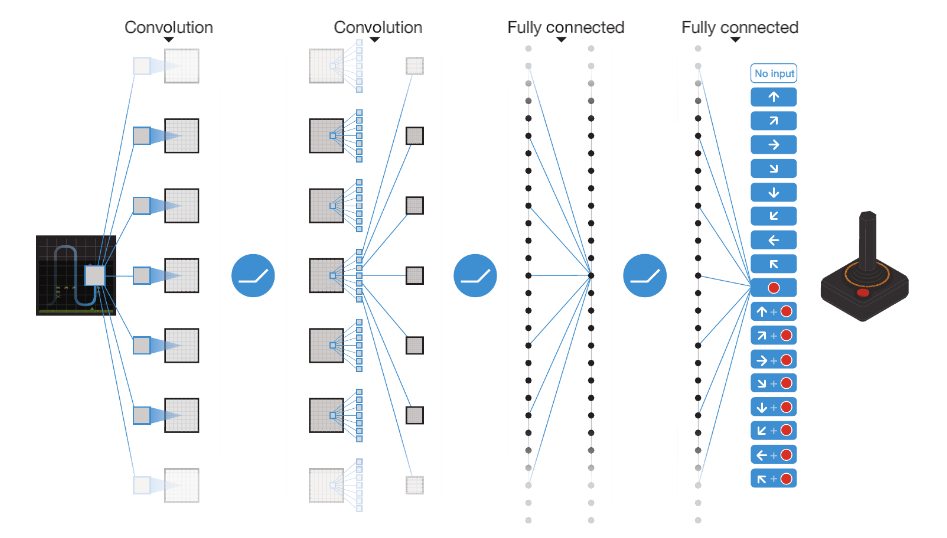
\includegraphics[width=1\linewidth]{network.png}
\caption{Deep Q-Network}
\label{network}
\end{figure}

Podstawą dla wykorzystywanych modeli jest DQN, Deep Q-Network opisana w pracy DeepMind na temat uczenia w grach Atari \cite{DeepMind:2015}. Jej architektura jest wizualizowana na rysunku \ref{network}. Można wyróżnić 3 usprawnienia ponad zwykłą sieć MLP która pozwoliły osiągnąć tak dobre wyniki:

\begin{itemize}
\item {Zastosowanie głębokiej sieci konwolucyjnej}
\item {Implementacji \textit{Odgrywania Doświadczeń (Experience Replay)}, co umożliwia sieci uczenie się na podstawie zapisanych wcześniej doświadczeń.}
\item {Użycie drugiej sieci ``celu'' do obliczania wartości funkcji akcji.}
\end{itemize}

Jak już zostało wspominane, wejściem do sieci są kolejne ramki z symulacji gry, przedstawione za pomocą tablicy pikseli. Jej rozmiar może być zmienny w zależności od środowiska, ale obraz z Ponga dostępny dzięki OpenAI ma rozmiar 210x160x3. W przetwarzaniu obrazów prym wiodą sieci konwolucyjne. Warstwy konwolucyjne w modelu mają za zadanie wyciągnięcie informacji z obrazu. 

Odgrywanie Doświadczeń polega na przechowywaniu doświadczeń modelu i losowe wybieranie z nich paczek do trenowania sieci. Doświadczenia są przechowywane jako krotki \textless stan, akcja, nagroda, następny stan\textgreater. Poprzez wykorzystywanie losowych wspomnień, zapobiegamy uczenia się jedynie tego co jest aktualnie wykonywane w środowisku i umożliwia uczenie na bardziej zróżnicowanych doświadczeniach. Przechowywana jest tylko wcześniej ustalona liczba doświadczeń, które są wraz z upływem kolejnych epok zastępowane nowszymi.

Sieć celu jest wykorzystywana do obliczenia wartości funkcji akcji, która to jest wykorzystywana do obliczenia straty każdej akcji podczas treningu. Innymi słowy służy jedynie do wyznaczenia która z dostępnych akcji jest według sieci optymalna. Niemożliwe jest wykorzystanie jednej sieci, która jednocześnie uaktualnia swoje wagi i generuje nowe wartości. Według cytowanej pracy, ze względu na ciągle zmieniające się wagi, które jednocześnie są pośrednio wykorzystywane do aktualizacji samych siebie (ponieważ wagi sieci wpływają na wynik funkcji akcji) sieć traci stabilność i przewidywane wartości mogą wymknąć się spod kontroli. Aby temu zapobiec, wagi sieci celu są stałe, jedynie co jakiś czas powoli aktualizowane do wag sieci bazowej.

Pracownicy DeepMind zaprezentowali kilka usprawnień do swojego podstawowego modelu. Pierwszym z nich jest określany pojęciem Double DQN \cite{DoubleDQN:2015}. Inspirowany faktem, że w podstawowym modelu często dochodziło do sytuacji, w której wartości funkcji akcji dla poszczególnych akcji w danym stanie były przeszacowane. Nie stanowiłoby to wielkiego problemu, jeśli wszystkie akcje byłyby przeszacowane w jednakowym stopniu, jednak badania potwierdzały, że było inaczej. Częste przyznawanie większych wartości funkcji akcji nieoptymalnym akcjom sprawiało, że model miał problemy z nauczeniem się odpowiedniego postępowania. Aby zapobiec tej sytuacji, autorzy zaproponowali, aby zamiast brać maksymalną wartość funkcji akcji wygenerowaną przez sieć celu(wykorzystywaną w trenowaniu sieci głównej), sieć główna jest wykorzystywana do generowania optymalnej akcji, a sieć celu generuje wartość funkcji akcji dla tej wybranej akcji. Poprzez oddzielenie generacji optymalnej akcji od generowania jej oceny, możemy znacznie przyśpieszyć i uregulować uczenie.

Drugim usprawnieniem jest Dueling DQN\cite{Dueling:2016}. Główną ideą jest rozbicie funkcji akcji na dwie osobne funkcje. Funkcja akcji określa, jak dobre jest podjęcie danej akcji w danym stanie - opisywana jest jako Q(s,a). Pierwszą składową tej funkcji jest funkcja wartości V(s), która określa, jaka jest wartość w przebywaniu w danym stanie. Drugą jest funkcja korzyści A(a), która określa o ile lepsze jest podjęcie danej akcji w porównaniu do innych. Ostatecznie:
\begin{equation}
\label{q2}
Q(s,a) = V(s) + A(a)
\end{equation}
Zaleta tego podejścia wynika z faktu, że nie w każdym momencie interesuje nas wartość i korzyść. Wykorzystując w przykładzie grę w ponga, w grze istnieją stany, w którym nie trzeba podejmować żadnej decyzji - dopiero odbiliśmy piłeczkę, porusza się ona w kierunku przeciwnika. Jesteśmy w dobrym stanie, nie ma więc sensu myśleć nad podjęciem jakiejkolwiek decyzji. Implementowane jest to przez rozdzielenie sieci na dwa przepływy, który każdy odpowiada za swoją funkcję i są na końcu łączone, co jest widoczne na rysunku \ref{dueling}.
\begin{figure}[h]
\centering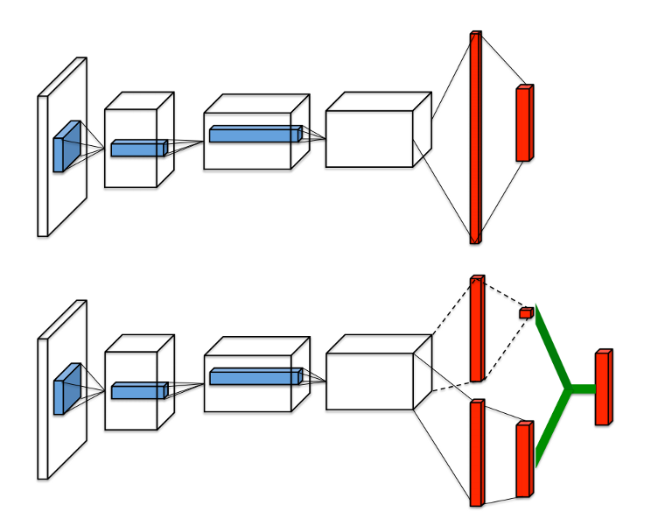
\includegraphics[width=1\linewidth]{dueling.png}
\caption{Dueling DQN}
\label{dueling}
\end{figure}

\section{Niektóre szczegóły implementacji}

Pierwsze postępy w implementacji modelu były oparte o poradnik \cite{implementation1} Dostępne w nim jest wprowadzenie do Q-learningu jak i do samego Tensorflowa. Początkowe rozdziały skupiają się na implementacji Q-learningu za pomocą tabel, jednak to rozwiązanie może być wykorzystywane tylko w najprostszych środowiskach. Następujące rozszerzenie do płytkich sieci neuronowych nie gwarantuje znacznej poprawy, ale stanowi punkt wejścia do stosowania sieci głębokich.

Dużym problemem była instalacja wszystkich zależności modelu - szczególnie Gym wymaga specyficznych warunków, umożliwiając działanie tylko z językiem Python i nie posiadając wsparcia dla systemu Windows. Konieczna była instalacja Linuxa i odpowiednia konfiguracja występujących na nim sterowników. Konieczna była instalacja interfejsu Cuda, który był niezbędny aby uczyć sieć na karcie graficznej - przyspieszając proces. Jest to istotne ze względu na to, że rozpatrywany problem wymaga często kilkudziesięciogodzinnego uczenia, nawet na wydajnych kartach graficznych. 

Przy instalacji wykorzystano platformę Anaconda, która umożliwia zarządzanie naukowymi bibliotekami do Pythona. Dodatkowym narzędziem był pip, pełniący podobną funkcję. 

Pierwsza implementacja DQN działała na prostym środowisku, aby można było szybko wyuczyć sieć i zauważyć wpływ parametrów na działanie sieci. Kontrolowany w nim był niebieski kwadrat i celem było dotarcie do zielonego kwadratu (nagroda +1) omijając jednocześnie czerwony kwadrat (nagroda - 1), co jest widoczne na rysunku\ref{proste}. Na początku każdego epizodu kwadraty były losowo układane na planszy 5x5.

\begin{figure}[h]
\centering
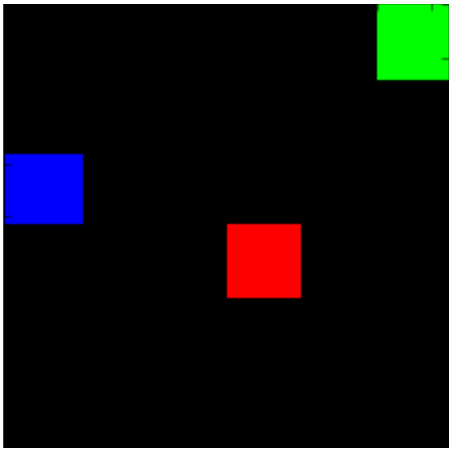
\includegraphics[width=0.4\linewidth]{testing.png}
\caption{Proste środowisko testowe}
\label{proste}
\end{figure}


Mimo że sieć w ciągu uczenia stale polepszała swoje działanie, co było obrazowane przez rosnącą średnią wartość nagrody, to na innych środowiskach, takich jak Pong, sieć nie wykazywała poprawy wraz z rosnącą liczbą epok. Ze względu na to, że istniejąca implementacja nie była napisana zbyt czytelnie, zdecydowano się na przetestowanie innej.

Przystosowano kolejną implementację z internetu\cite{implementation2}. W podanym repozytorium dostępna jest implementacja podstawowej wersji sieci oraz wariantu z rozszerzeniem Dueling. Oparta jest o interfejs Keras działający na bibliotece TensorFlow. Korzysta również z biblioteki Gym od OpenAI, co umożliwia prostą wymianę gry na której uczona jest sieć. Konieczne było jedynie zaktualizowanie projektu na nowe wersje TensorFlowa i Kerasa. Po tych modyfikacjach uruchomiono uczenie na grze Breakout, w której celem jest sterowanie paletką tak, aby odbijać nadlatującą piłkę w celu niszczenia klocków znajdujących się u góry ekranu. Zobrazowanie widoczne jest na rysunku \ref{breakout}. Niestety, ze względu na ograniczenia czasowe uruchomiono uczenie jedynie na 8 godzin, co nie pozwoliło na weryfikację działania. Artykuły wskazują, że wzrost nagrody występuje dopiero po tym okresie. Jednak inne parametry zachowywały się zgodnie z przewidywaniami - ciągle rosły średnie wartości funkcji akcji sugerując ich modyfikację. Dopiero po pewnym czasie te wartości osiągnęły by taki układ, który pozwala na podejmowanie odpowiednich decyzji.

\begin{figure}[h]
\centering
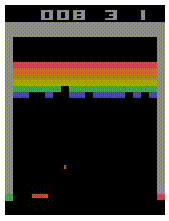
\includegraphics[width=0.4\linewidth]{test2.png}
\caption{Gra Breakout}
\label{breakout}
\end{figure}

\section{Podsumowanie}

Mimo niepowodzenia w kompletnym przetestowaniu modelu, można z projektu wyciągnąć pewne wnioski. Po pierwsze, testowanie DQN na prostym środowisku jest przydatne do optymalizacji parametrów, ale nie może wiarygodnie służyć do przewidywania działania na bardziej skomplikowanym środowisku. Co więcej, aby przetestować działanie sieci w domowych warunkach, konieczna jest implementacja możliwości zapisywania i wczytywania stanu sieci aby móc wznowić uczenie w czasie, gdy dostępne są do tego środki. Innym rozwiązaniem jest posiadanie dedykowanej maszyny. 

Dodatkowo, praca z Kerasem okazała się dużo prostsza niż z samym TensorFlowem. Może nie jest to twierdzenie odkrywcze, ale używając jego od początku, można znacznie przyspieszyć zrozumienie modelu ułatwiając modyfikacje. 


%% The Appendices part is started with the command \appendix;
%% appendix sections are then done as normal sections
%% \appendix

%% \section{}
%% \label{}

%% References
%%
%% Following citation commands can be used in the body text:
%% Usage of \cite is as follows:
%%   \cite{key}          ==>>  [#]
%%   \cite[chap. 2]{key} ==>>  [#, chap. 2]
%%   \citet{key}         ==>>  Author [#]

%% References with bibTeX database:

\bibliographystyle{model1-num-names}
\bibliography{sample}

%% Authors are advised to submit their bibtex database files. They are
%% requested to list a bibtex style file in the manuscript if they do
%% not want to use model1-num-names.bst.

%% References without bibTeX database:

% \begin{thebibliography}{00}

%% \bibitem must have the following form:
%%   \bibitem{key}...
%%

% \bibitem{}

% \end{thebibliography}


\end{document}

%%
%% End of file `elsarticle-template-1-num.tex'.
